\documentclass{cmc}

\begin{document}

\pagestyle{fancy}
\lhead{\textit{\textbf{Computational Motor Control, Spring 2025} \\
    Python exercise, Lab 2, NOT GRADED}} \rhead{Student \\ Names}

\section*{Student names: \ldots (please update)}

\textit{Instructions: Update this file (or recreate a similar one, e.g.\ in
  Word) to prepare your answers to the questions. Feel free to add text,
  equations and figures as needed. Hand-written notes, e.g.\ for the development
  of equations, can also be included e.g.\ as pictures (from your cell phone or
  from a scanner).  \textbf{This lab is not graded. However, the lab exercises
    are meant as a way to familiarise with dynamical systems and to study them
    using Python to prepare you for the final project.} This file does not need
  to be submitted and is provided for your own benefit. The graded exercises
  will have a similar format.}

\textit{The file \fileref{lab\#.py} is provided to run all exercises in
  Python. Each \fileref{exercise\#.py} can be run to run an exercise
  individually. The list of exercises and their dependencies are shown in
  Figure~\ref{fig:files}. When a file is run, message logs will be printed to
  indicate information such as what is currently being run and and what is left
  to be implemented. All warning messages are only present to guide you in the
  implementation, and can be deleted whenever the corresponding code has been
  implemented correctly.}

\begin{figure}[ht]
  \centering 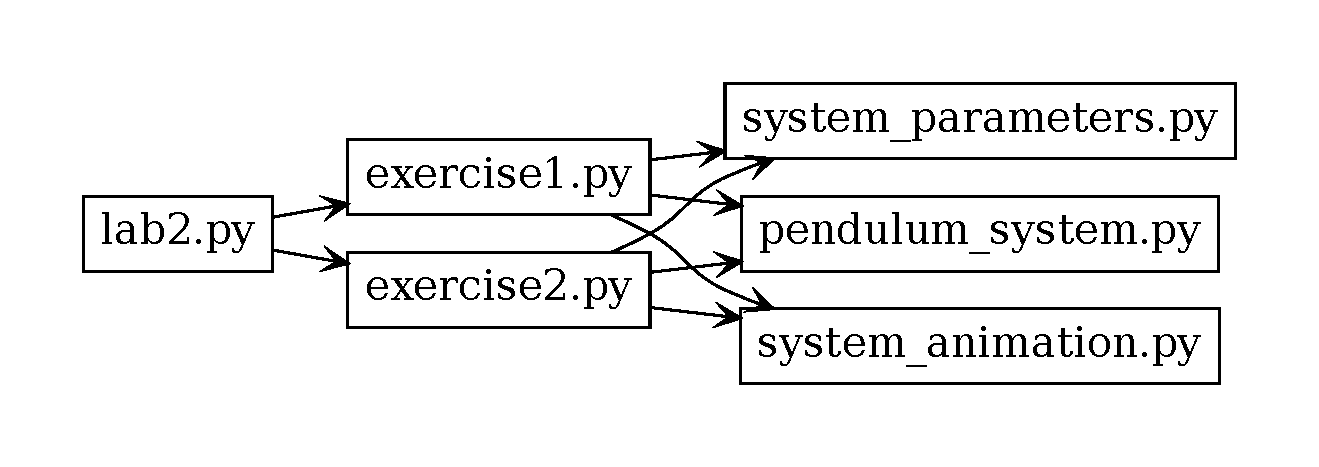
\includegraphics[width=0.5\textwidth]{figures/files}
  \caption{\label{fig:files} Exercise files dependencies. In this lab, you will
    be modifying \fileref{exercise1.py}, \fileref{exercise2.py} and \fileref{pendulum\_system.py}.
    }
\end{figure}

\textit{In this exercise, you will explore the different modeling
  techniques that can be used to control a single joint and
  segment. We initially start by exploring a single joint controlled
  by a a single simplified pendulum model with damping(friction) (exercise1)
  and then extend it to pair of spring-dampers muscle models (exercise2).
  These only represent the passive dynamics observed in a real musculoskeletal system.
  You are provided with a code that can simulate a pair spring-damp muscle model
  . }

\textbf{Important note:}
\textit{Both exercise use a generic class that can handle both a pair of
		spring damp muscles, or a single spring damp muscle sketched in Figure
		\ref{fig:spring_mass_damper_sketch}. Each muscle pair
		contains sping constants and resting angles, and damping coefficients.
		Simply set all the values of these parameters equal for the two pairs
		to study the behavior of a single spring-damper instead of a pair (in Exercise 1).
		Have a look at the specification of parameters of the pendulum
		system in the class \textit{PendulumParameters} in \fileref{system\_parameters.py}.}


\begin{figure}[ht]
  \centering 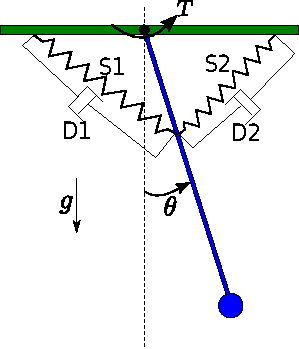
\includegraphics[width=0.2\textwidth]{figures/pendulum_spring_damper}
  \caption[pendulum with spring]{Pendulum model with two springs S1
    and S2 and two dampers b1 and b2\\
    $T$ - Positive torque direction.\\
    $g$ - Gravity.\\
    $\theta$ - Angle made by the pendulum
    \label{fig:spring_mass_damper_sketch} }
\end{figure}


 % ===== exercise 1 ======

\section*{Question 1: Pendulum with friction}

\subsection*{1.a Find the fixed points of the pendulum with friction
  (i.e. damping, and analyze their stability using a local linearization
  under no external input $T_{ext}=0$ ) expressed in the following equation
  (briefly describe the calculation steps). }


\begin{equation}
  \label{eq:ode-pendulum}
  I\ddot{\theta} = -mgLsin(\theta) + T_{ext} - b \dot{\theta}
\end{equation}

Considering Inertia $I = mL^2$, the equation of the pendulum can be
written as,

\begin{equation}
  \label{eq:pendulum}
  \ddot{\theta} = -g\frac{sin(\theta)}{L} + \frac{T_{ext}}{I} - b \frac{\dot{\theta}}{I}
\end{equation}

where $\theta$ is the angle, $g$ the gravity constant, $L$ the length of the pendulum
and $b$ is the damping coefficient.


\subsection*{1.b Implement the the damping equation of the pendulum using equations described above in the function
  \fileref{pendulum\_system.py::pendulum\_equation}. Numerically solve the differential equations of the pendulum
  with different initial conditions.  Show several time evolutions and phase
  portraits with different initial conditions that illustrate several aspects of
  the interesting behavior of the pendulum. Additionally, implement the damping parameter and demonstrate examples of underdampded, critically damped and overdamped behaviors.
  See \fileref{exercise1.py} and \fileref{system\_parameters.py} and
  \fileref{pendulum\_system.py} for help with implementation.}


\subsection*{1.c Investigate and describe how the behavior of the pendulum
  changes if friction is zero (b=0).  Show a new phase portrait.}


\subsection*{1.d Does the pendulum without friction (b=0) produce stable limit
  cycles? Discuss, and try to support your statement with some numerical
  simulations (show figures) and/or analytical arguments.}


\subsection*{1.e Investigate how the behavior of the pendulum changes if the
  viscous friction term is replaced with a dry (Coulomb) friction term. Unlike
  viscous friction, dry friction does not depend on speed, only the direction of
  movement. What are the main differences between the two types of pendulum?
  (discuss and show some examples). And is there anything notable about the
  numerical integration of the pendulum with dry friction? If yes, what and why?}

\begin{equation}
  \label{eq:ode-pendulum-dry}
  \ddot{\theta} = - {g \over L} \sin \theta - b \cdot sign(\dot{\theta})
\end{equation}





 % ===== exercise 2 ======

\section*{Exercise 2 : Pendulum model with passive elements}
\label{sec:question-1}

Mechanical behavior of muscle tissue can be approximated by simple
passive elements such as springs and dampers. These elements, when
combined properly, allow to study the behavior of muscle under
compressive and tensile loads.

Consider the following equation describing the motion of simple
pendulum with an external torque $T_{ext}$,

\begin{equation}
  \label{eq:pendulum_1}
  I\ddot{\theta} = -mgLsin(\theta) + T_{ext}
\end{equation}


Consider the system only for the pendulum range $\theta$ =
$[-\pi/2, \pi/2]$

\subsection*{Explore the pendulum model with two antagonist spring
  elements}

In this question the goal is to add two antagonist springs to the
pendulum model which you are already familiar with from lab 2
exercises. For simplicity we assume the springs directly apply a
torsional force on to the pendulum.  Use equation \ref{eqn:spring} to
develop the spring model.

\textit{\textbf{Note} : The springs can only produce force in
  one-direction like the muscles.  That is, they can only apply a
  pulling force and apply a zero force when compressed.  In terms of
  torsion this translates to, spring S1 can exert only clockwise
  torque and spring S2 can exert only counter-clockwise torque.  You
  need to accommodate for this condition in the equations shown below.}

The setup for the pendulum with a pair of antagonist springs is as
shown in figure \ref{fig:pendulum_spring}. Use \fileref{exercise2.py},
\fileref{pendulum\_system.py} and \fileref{system\_parameters.py} files to
complete the exercise.


\begin{figure}[H]
  \centering
  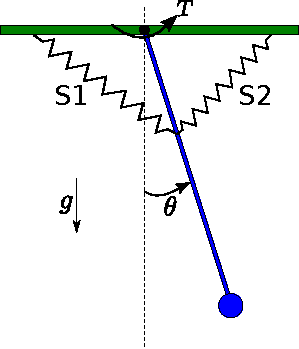
\includegraphics[width=.3\textwidth]{figures/pendulum_spring}
  \caption[pendulum with spring]{Pendulum model with two springs S1
    and S2.\\
    $T$ - Positive torque direction.\\
    $g$ - Gravity.\\
    $\theta$ - Angle made by the pendulum}
  \label{fig:pendulum_spring}
\end{figure}


\begin{equation}
  \label{eqn:spring}
  T_{S} = k \cdot (\theta_{ref} - \theta)
\end{equation}

Where,
\begin{itemize}
\item $T_{S}$ : Torsional Spring force
\item $k$ : Spring Constant
\item $\theta_{ref}$ : Spring reference angle
\item $\theta$ : pendulum angle
\end{itemize}

Substituting the above in \ref{eq:pendulum},

\begin{eqnarray}
  \label{eq:spring}
  \ddot{\theta} = -g\frac{sin(\theta)}{L} + \frac{T_{ext}}{I} + \frac{T_{S}}{I} \\
  \ddot{\theta} = -g\frac{sin(\theta)}{L} + \frac{T_{ext}}{I} + \frac{k \cdot (\theta_{ref} - \theta)}{I} \label{eq:genSpring}
\end{eqnarray}

Use the generalized form of the spring equation described in
\ref{eq:genSpring} to extend it to both the antagonist springs S1 and
S2 with the necessary conditions to make sure springs do not produce
when compressed.



\subsection*{2.a Implement the dynamic equations of the pendulum with
  springs using equations described above in the function
  \fileref{pendulum\_system.py::pendulum\_equation}.  Does the system
  have a stable limit cycle behavior?  Describe and run an experiment
  to support your answer. You can use the function
  \fileref{exercise2.py::pendulum\_perturbation} to perturb the
  pendulum either by changing states or applying an external torque.
  Use the class \fileref{system\_animation.py::SystemAnimation} to
  visualize the pendulum. Example code can be found in
  \fileref{exercise2.py::exercise2}}
\label{subsec:2.a}


\subsection*{2.b Explore the role of spring constant ($k$) and spring
  reference angle ($\theta_{ref}$) in terms of range of motion,
  amplitude and frequency of pendulum. Keep the constants equal, i.e
  $k_1$  = $k_2$ and $\theta_{ref1} = \theta_{ref2}$
  \\ Refer to \fileref{exercise2.py::exercise1} for an example}


\subsection*{2.c Explain the behavior of the model when you have
  asymmetric spring constants ($k$) and spring reference angles
  ($\theta_{ref}$), i.e. $k_1 \neq k_2$ and $\theta_{ref1} \neq \theta_{ref2}$
  Support your responses with relevant plots}


\subsection*{Explore the pendulum model with two antagonist spring and damper elements}
Over time muscles lose energy while doing work. In order to account
for this property, let us now add a damper in parallel to the spring
model. Use equation \ref{eqn:damper} to develop the damper model.

\textit{\textbf{Note} : Like the previous springs, the springs in spring-dampers
  can only produce a force in one-direction.  However, the damper terms do not
  have this limitation and each damper can exert a force in both directions.}

Again use \fileref{exercise2.py}, \fileref{pendulum\_system.py} and
\fileref{system\_parameters.py} files to complete the exercise. The
setup for the pendulum model with a pair of antagonist spring and
dampers in parallel is as shown in figure
\ref{fig:pendulum_spring_damper}.


\begin{figure}[H]
  \centering
  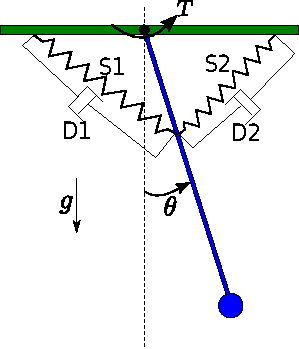
\includegraphics[width=.3\textwidth]{figures/pendulum_spring_damper}
  \caption[pendulum with spring]{Pendulum model with two springs S1
    and S2 and two dampers b1 and b2\\
    $T$ - Positive torque direction.\\
    $g$ - Gravity.\\
    $\theta$ - Angle made by the pendulum}
  \label{fig:pendulum_spring_damper}
\end{figure}



\begin{equation}
  \label{eqn:damper}
  T_{B} = b \cdot \dot{\theta}
\end{equation}

Where,
\begin{itemize}
\item $T_{B}$ : Torsional Damper force
\item $b$ : Damping Constant
\item $\dot{\theta}$ : pendulum angular velocity
\end{itemize}

The combined spring damper torque is given by,
\begin{equation}
  \label{eq:spring_damper}
  T_{S} - T_{B} = k \cdot (\theta_{ref} - \theta) - b \cdot \dot{\theta}
\end{equation}

The minus for the damper comes from the fact that damper is acting
against the work done by the spring.

Substituting the above in \ref{eq:pendulum}

\begin{eqnarray}
  \label{eq:spring-damper}
  \ddot{\theta} = -g\frac{sin(\theta)}{L} + \frac{T_{ext}}{I} + \frac{T_{S} - T_{B}}{I} \\
  \ddot{\theta} = -g\frac{sin(\theta)}{L}+ \frac{T_{ext}}{I} + (\frac{k \cdot (\theta_{ref} - \theta) - b \cdot \dot{\theta}}{I}) \label{eq:genSpringDamper}
\end{eqnarray}

Use the generalized form of the spring equation described in
\ref{eq:genSpringDamper} to extend it to both the antagonist
spring-damper systems (S1-D1) and (S2-D2).


\subsection*{2.d Implement the dynamics equations of the pendulum to
  now include the damping using the equations described above. Modify
  \fileref{pendulum\_system.py::pendulum\_equation}.  How does the
  behavior now change compared to the pendulum without dampers? Briefly explain and support your
  responses with relevant plots}


\subsection*{2.e Can you find a combination of spring constants ($k$),
  damping constants ($b$) and spring reference angles ($\theta_{ref}$)
  that makes the pendulum rest in a stable equilibrium at
  ($\theta = \pi/6$) radians? Describe how you arrive at the necessary
  parameters and support your response with relevant plots.}


\subsection*{2.f What is the missing component between a real muscle
  and the muscle model with passive components that you just explored?
  What behavior's do you lack because of this missing component?}



\end{document}